% file: ColdnetTopKnots.tex
% Cold neutrons and Topological Knots
% 
% github        : ernestyalumni
% gmail         : ernestyalumni 
% linkedin      : ernestyalumni 
% wordpress.com : ernestyalumni
%
% This code is open-source, governed by the Creative Common license.  Use of this code is governed by the Caltech Honor Code: ``No member of the Caltech community shall take unfair advantage of any other member of the Caltech community.'' 

\documentclass[10pt]{amsart}
\pdfoutput=1
\usepackage{mathtools,amssymb,lipsum,caption}

\usepackage{graphicx}
\usepackage{hyperref}
\usepackage[utf8]{inputenc}
\usepackage{listings}
\usepackage[table]{xcolor}
\usepackage{pdfpages}
\usepackage{tikz}
\usetikzlibrary{matrix,arrows}

\usepackage{multicol}

\hypersetup{colorlinks=true,citecolor=[rgb]{0,0.4,0}}


%\oddsidemargin=15pt
%\evensidemargin=5pt
%\hoffset-45pt
%\voffset-55pt
%\topmargin=-4pt
%\headsep=5pt
%\textwidth=1120pt
%\textheight=595pt
%\paperwidth=1200pt
%\paperheight=700pt
%\footskip=40pt








\newtheorem{theorem}{Theorem}
\newtheorem{corollary}{Corollary}
%\newtheorem*{main}{Main Theorem}
\newtheorem{lemma}{Lemma}
\newtheorem{proposition}{Proposition}

\newtheorem{definition}{Definition}
\newtheorem{remark}{Remark}

\newenvironment{claim}[1]{\par\noindent\underline{Claim:}\space#1}{}
\newenvironment{claimproof}[1]{\par\noindent\underline{Proof:}\space#1}{\hfill $\blacksquare$}

%This defines a new command \questionhead which takes one argument and
%prints out Question #. with some space.
\newcommand{\questionhead}[1]
  {\bigskip\bigskip
   \noindent{\small\bf Question #1.}
   \bigskip}

\newcommand{\problemhead}[1]
  {
   \noindent{\small\bf Problem #1.}
   }

\newcommand{\exercisehead}[1]
  { \smallskip
   \noindent{\small\bf Exercise #1.}
  }

\newcommand{\solutionhead}[1]
  {
   \noindent{\small\bf Solution #1.}
   }


\title{Cold Neutrons and Topological Knots}
\author{Ernest Yeung \href{mailto:ernestyalumni@gmail.com}{ernestyalumni@gmail.com}}
\date{22 avril 2016}
\keywords{Cold neutrons, Ultracold neutrons, Knot homology, Knot polynomials, Chern-Simons theory, theta angle, $\theta$-angle, quantum field theory, gauge theory, topological gauge theory}

\begin{document}

\definecolor{darkgreen}{rgb}{0,0.4,0}
\lstset{language=Python,
 frame=bottomline,
 basicstyle=\scriptsize,
 identifierstyle=\color{blue},
 keywordstyle=\bfseries,
 commentstyle=\color{darkgreen},
 stringstyle=\color{red},
 }
%\lstlistoflistings

\maketitle

\tableofcontents

%\begin{multicols*}{2}

\begin{abstract}
We investigate exact solutions, via topological gauge theory and knot polynomials, or knot homologies, applied to ultracold neutrons in beta decay, in particular, via the $\theta$-term in the Lagrangian describing neutrons.  
\end{abstract}


\part{(Weekly) reports}

\subsection{20160422 Things to do}

Clarify Manifold setup $\partial M \hookrightarrow M$; explore various manifold setups; pdf or equation of motion out of $\mathcal{L}$ and Euler-Lagrange equation and compare those equations to instanton equations of Gaiotto and Witten (2011) \cite{GW2011}; understand Virasoro algebra and conformal blocks for the quantum ``states'' that we can act upon; read more: Gaiotto and Witten (2011) \cite{GW2011}; Gukov (2007) \cite{Guko2007}, and of course classic Witten (1988) \cite{Witten:1988hf}

\part{Introduction}

\section{Geometry; Geometric setup; Manifold setup}

Following Eq. 1.28 on pp.5 of Subsection 1.3 The $\theta$-term of Hickerson (2013) \cite{Hick2013}, for a 3-cylinder $\partial M$, he has the following setup:
\[
\partial M = \mathbb{D}^3(t^+) \bigcup \mathbb{D}^3(t^-) \bigcup \mathbb{S}^2 \times \mathbb{R}
\]
Let's count dimensions.  
\[
\text{dim} \partial M  = \text{dim} \mathbb{D}^3(t^+) + \text{dim}\mathbb{S}^2 + 1 
\]
Now $\text{dim}\mathbb{S}^2 =2$.  So do we have more dimensions than alloted?  

Let's account for the various setups for a 4-dimensional topological gauge theory that involves knot polynomials (i.e. knot homologies).  It appears that Gaiotto and Witten (2011) \cite{GW2011} likes to include Riemann surfaces in $\partial M$, so there setup could be
\[
\partial M = \mathbb{C} \times \mathbb{R} (\text{or } \mathbb{C}\times S^1 (???) )
\]
where $\mathbb{C} \equiv $ Riemann surface (i.e. $f:\mathbb{C} \to \mathbb{C}$, $f$ holomorphic, i.e. $\begin{aligned} & \quad \\
  & \frac{ \partial f}{ \partial \overline{z}} = 0 \\
  & \frac{ \partial \overline{f}}{ \partial z } = 0 \end{aligned}$).  


knot $K$ is an embedding $f: S^1 \to S^3$

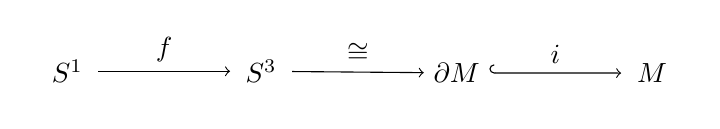
\begin{tikzpicture}
  \matrix (m) [matrix of math nodes, row sep=3.8em, column sep=4.8em, minimum width=2.2em]
  {
S^1 & S^3 & \partial M & M \\
};
  \path[->]
  (m-1-1) edge node [auto] {$f$} (m-1-2)
  (m-1-2) edge node [auto] {$\cong $} (m-1-3)
  ;
  \path[right hook->]
  (m-1-3) edge node [auto] {$i$} (m-1-4)
  ;
\end{tikzpicture}

Let us follow Hickerson (2013) \cite{Hick2013} to understand the number of approaches and models for ultracold neutrons \cite{Hick2013}.  

Consider the term
\[
\mathcal{L}_{\theta} = \frac{ \theta g^2}{ 8 \pi^2 } \text{tr}(F\wedge F) = \frac{ \theta g^2}{8 \pi^2} d\text{tr}( A \wedge dA + \frac{2}{3} A \wedge A \wedge A)
\]

We've seen how 
\begin{equation}
  \text{tr}(F_A \wedge F_A) \equiv \text{tr}(F\wedge F) = d\text{tr}(A \wedge dA + \frac{2}{3} A \wedge A \wedge A )
\end{equation}
is true, without regards to a \emph{metric} $g$ (or i.e. \emph{metric bundle} $g$ over $M$).  In pp. 5 Subsection 1.3 The $\theta$-term of Hickerson (2013) \cite{Hick2013}, the dual to $F$ was utilized.  Let's avoid utilizing ``electric-magnetic'' dual, or $g$, or Hodge dual terms in order to think purely ``topologically.''




\part{Preliminaries; (review of) Elementary concepts}


\section{Curvature}

Consider a principal-$G$ bundle with Lie group $G$, $P\xrightarrow{ \pi } M$.  Note that an associated bundle, a vector bundle, can be constructed from principal $G$-bundle $P$, through representation $\rho : G \to Gl(n;\mathbb{K})$ (cf. 10.9 Associated vector bundles of Taubes (2011) \cite{CTaubes2011}), in that 
\[
\begin{gathered}
\begin{tikzpicture}
  \matrix (m) [matrix of math nodes, row sep=3.8em, column sep=4.8em, minimum width=2.2em]
  {
P  \\
M  \\
};
  \path[->]
  (m-1-1) edge node [left] {$\pi$} (m-2-1)
  ;
\end{tikzpicture} \xrightarrow{ \rho : G \to \text{Gl}(n;\mathbb{K})} P \times_{\rho} \mathbb{K}^n \equiv P\times \mathbb{K}^n/(p,v)\sim (pg^{-1}, \rho(g)v) \quad \, \forall \, g \in G
\end{gathered}
\]
for $\mathbb{K} = \mathbb{R} \text{ or } \mathbb{C}$ and $\mathbb{K}^n$ being a vector space of dimension $n$ over field $\mathbb{K}$. 

Recall the exterior covariant derivative $D$ s.t.
\[
\begin{aligned}
  & D: \Omega^p(M;E) \to \Omega^{p+1}(M;E) \\ 
  & D(\theta \otimes s) = d\theta \otimes s + (-1)^p \theta \wedge \nabla s = d\theta \otimes s + \nabla s \wedge \theta
\end{aligned}
\]
with $E \xrightarrow{\pi} M$ being a vector bundle (from which one can construct the principal $G$ bundle, if so desired).  


\begin{proposition}
  For exterior covariant derivative $D: \Omega^p(M;E) \to \Omega^{p+1}(M;E)$, $\forall \, \eta \in \Omega^p(M;E)$, 
\[
D^2 \eta \equiv D\circ D \eta = F\wedge \eta
\]
where $F \in \Omega^p(M; \text{End}(E))$, and $F$ \emph{unique}
\end{proposition}

\begin{proof}
$\forall \, \eta \in \Omega^p(M;E)$, of the form $\eta = \theta \otimes s$, where $\theta \in \Omega^p(M)$, $s\in \Gamma(E)$, 
\[
\begin{gathered}
  D\eta = d\theta \otimes s + (-1)^p \theta \wedge \nabla s = d\theta \otimes s + (-1)^p \theta \wedge (ds + \omega^k_{ \; \; i } s^i e_k) = d\theta \otimes s + ds \wedge \theta + \omega^k_{ \; \; i} s^i \wedge \theta \otimes e_k = \\
  = (s^k d\theta + ds^k \wedge \theta + \omega^k_{ \; \; i } s^i \wedge \theta ) \otimes e_k 
\end{gathered}
\]
\[
\begin{gathered}
  D\circ D \eta \equiv DD\eta = (ds^k \wedge d\theta + (-1)ds^k \wedge d\theta + ds^i \wedge \omega^k_{ \; \; i} \wedge \theta + s^i d\omega^k_{ \; \; i } \wedge \theta + (-1) \omega^k_{ \; \; i} s^i \wedge d\theta ) \otimes e_k +\\
  + (-1)^{p+1}(s^k d\theta + ds^k \wedge \theta + \omega^k_{ \; \; i} s^i \wedge \theta ) \otimes \wedge \omega^l_{ \; \; k} e_l = \\
  = (ds^i \wedge \omega^l_{ \; \; i} \wedge \theta + s^i d\omega^l_{ \; \; i} \wedge \theta + (-1) \omega^l_{ \; \; i} s^i \wedge d\theta ) \otimes e_l + \\
  + (s^k \omega^l_{ \; \; k} \wedge d\theta + \omega^l_{ \; \; k } \wedge ds^k \wedge \theta + \omega^l_{ \; \; k} \wedge \omega^k_{ \; \; i } s^i \wedge \theta ) e_l = \\
  = (d\omega^l_{ \; \; i} + \omega^l_{ \; \; k } \wedge \omega^k_{ \; \; i} )s^i \wedge \theta e_l
\end{gathered}
\]
If you're following at home (i.e. independent study), one only needs to be careful with factors of $(-1)$ when ``commuting through'' the wedge product $\wedge$.  

I (still) find it a near miracle that terms cancel such that $F$ takes this form (with, simply a change of notation, $\omega \equiv A$):
\[
F = dA + A\wedge A \in \Omega^p(M;\text{End}E)
\]
By Lemma 11.1 of Sec. 11.2 the space of covariant derivatives of Taubes (2011) \cite{CTaubes2011}, this $F$ is \emph{unique}.  

Thus
\[
D^2 \eta = F \wedge \eta 
\]
for, notice that for, locally (in components)
\[
A = A^k_{ \; \; ij} dx^j \otimes (e_k \otimes e^i)
\]
\[
\begin{gathered}
  F = dA + A \wedge A = \frac{ \partial A^k_{ \; \; lj} }{  \partial x^i } dx^i \wedge dx^j \otimes (e_k \otimes e^l) + A^k_{  \; \; mi } A^m_{ \; \; lj } dx^i \wedge dx^j \otimes (e_k \otimes e^l) = \\
  = \left( \frac{ \partial A^k_{ \; \; lj} }{ \partial x^i} + A^k_{ \; \; mi} A^m_{ \; \; lj } \right) dx^i \wedge dx^j \otimes (e_k \otimes e^l )
\end{gathered}
\]
and so
\[
F\wedge \eta = \left( \frac{ \partial A^k_{ \; \; lj} }{ \partial x^i } + A^k_{ \; \; mi} A^m_{ \; \; lj } \right) dx^i \wedge dx^j \wedge \theta \otimes e_k s^l
\]
\end{proof}

\subsubsection{Alternative form of curvature $F$ in terms of commutators}
cf. Subsection 12.6 Curvature and commutators of Taubes (2011) \cite{CTaubes2011}.  

Consider $\forall \, U,V \in \mathfrak{X}(M)$, $X\in \Gamma(E)$,
\[
\nabla_U X = U^j \left( \frac{ \partial X}{ \partial x^j} + A^k_{ \; \; ij} X^i \right) = U^j \left( \frac{ \partial }{ \partial x^j } + A_j \right) X \in \Gamma(E)
\]
and so clearly 
\[
\nabla_U \in \Gamma(\text{End}(E))
\]
Also recall the commutator for vector fields, in component form (locally):
\[
[U,V] = \left( U^i \frac{ \partial }{ \partial x^i} V^j -  V^i \frac{ \partial }{ \partial x^i} U^j \right) \frac{ \partial }{ \partial x^j} \in \mathfrak{X}(M)
\]
and so 
\[
\nabla_{[U,V]} = \left( U^i \frac{ \partial }{ \partial x^i } V^j - V^i \frac{ \partial }{ \partial x^i } U^j \right) \left( \frac{ \partial }{ \partial x^j } + A_j \right)
\]
Consider that 
\[
\begin{gathered}
\nabla_U \nabla_V = \\
 = U^i \left[ \left( \frac{ \partial }{ \partial x^i } + A_i \right) V^j \left( \frac{ \partial }{ \partial x^j} + A_j \right) \right] = \\
  = U^i \left[  \frac{ \partial V^j}{ \partial x^i} \left( \frac{ \partial }{ \partial x^j} + A_j \right) + V^j \left( \frac{ \partial^2}{ \partial x^i \partial x^j } + \frac{ \partial A_j }{ \partial x^i } + A_j \frac{ \partial }{ \partial x^i } \right) + A_i V^j \frac{ \partial }{ \partial x^j} + A_i V^j A_j \right]
\end{gathered}
\]
Then by canceling out matching terms, 
\[
\begin{gathered}
  [ \nabla_U, \nabla_V ] - \nabla_{[U,V] } = U^i V^j \frac{ \partial A_j}{ \partial x^i} - V^i U^j \frac{ \partial A_j}{ \partial x^i} + U^i V^j A_i A_j - V^i U^j A_i A_j = \\
  = \left( \left( \frac{ \partial A_j }{ \partial x^i } - \frac{ \partial A_i}{ \partial x^j} \right) + [A_i, A_j] \right) U^i V^j = F(U,V)
\end{gathered}
\]
and so we have this form for the curvature $F(U,V) \in \Gamma(\text{End}(E))$, $\forall \, U,V \in \mathfrak{X}(M)$, 
\[
F(U,V) = \left( \left( \frac{ \partial A_j}{ \partial x^i } - \frac{ \partial A_i}{ \partial x^j } \right) + [A_i,A_j] \right)U^i V^j
\]
but I think that one should keep in mind that this is just one form that $F$ could take, if it is applied to $U,V$ beforehand.  

\subsubsection{deRham cohomology}

I'm going to now follow Section 12.2 Closed forms, exact forms, diffeomorphisms and De Rham cohomology of Taubes (2011) \cite{CTaubes2011}.  

Recall the definition of \emph{deRham cohomology}:
\begin{equation}
  H^p_{\text{deRham}}(M) := \text{ker}d/\text{im}d \qquad \, \left( = \lbrace \omega | d\omega = 0 \rbrace / \lbrace \theta | \theta = d\alpha \text{ for } \alpha \in \Omega^{p-1}(M) \rbrace \right)
\end{equation}

If $M,N$ smooth manifolds, smooth map $f: M \to N$, $\forall \, \alpha \in \Omega^{p-1}(N)$, then
\begin{equation}
  f^*(d\alpha ) =d(f^*\alpha) \text{ or } f^* d = df^*
\end{equation}
i.e.
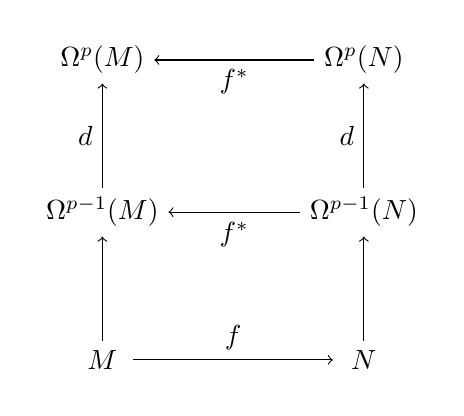
\begin{tikzpicture}
  \matrix (m) [matrix of math nodes, row sep=3.8em, column sep=4.8em, minimum width=2.2em]
  {
\Omega^p(M) & \Omega^p(N)  \\
\Omega^{p-1}(M) & \Omega^{p-1}(N)  \\
M & N   \\
};
  \path[->]
  (m-1-2) edge node [auto] {$f^*$} (m-1-1)
  (m-2-1) edge node [auto] {$d$} (m-1-1)
  (m-2-2) edge node [auto] {$d$} (m-1-2)
  edge node [auto] {$f^*$} (m-2-1)
  (m-3-1) edge node [auto] {$$} (m-2-1)
  edge node [auto] {$f$} (m-3-2)
  (m-3-2) edge node [auto] {$$} (m-2-2)
  ;
\end{tikzpicture}
\begin{proof}
Indeed, this can be shown, by considering local expressions: locally, $\alpha_I dy^I \in \Omega^{p-1}_y(N)$ where $I \equiv (i_1, i_2 \dots i_{p-1})$ s.t. $i_1 < i_2 < \dots < i_{p-1}$, and consider, with $f(x)=y$:
\[
\begin{gathered}
  \begin{aligned}
    & d\alpha = \frac{ \partial \alpha_I}{ \partial y^i} dy^i \wedge dy^I = \frac{ \partial \alpha_I}{\partial y^i} \epsilon^{iI }_J dy^J \text{ since there's only 1 way to permute $iI$ into $J=(j_1 \dots j_p)$ s.t. $j_1 < \dots < j_p$ } \\ 
    & f^*d\alpha = \frac{ \partial \alpha_I}{ \partial y^i} \epsilon^{iI}_J \frac{ \partial y^J}{ \partial x^k} dx^k \\ 
    & f^*\alpha = \alpha_I \frac{ \partial y^I}{ \partial x^J} dx^J = \frac{ \partial \alpha_I}{ \partial y^i} \frac{ \partial y^i }{ \partial x^j} \frac{ \partial y^I}{ \partial x^J} \epsilon^{jJ}_K dx^K
\end{aligned}
\end{gathered}
\]
Now
\[
\begin{gathered}
  df^* \alpha = \left( \frac{ \partial \alpha_I}{ \partial x^i} \frac{ \partial y^I}{ \partial x^j} + \alpha_I \frac{ \partial^2 y^I }{ \partial x^i \partial x^J} \right) dx^i \wedge dx^J = \left( \frac{ \partial \alpha_I}{ \partial x^i} \frac{ \partial y^I}{ \partial x^J} + \alpha_I \frac{ \partial^2 y^I}{ \partial x^i \partial x^J} \right) \epsilon^{iJ}_K dx^K = \\
  = \frac{ \partial \alpha_I}{ \partial y^i} \frac{ \partial y^i}{ \partial x^j} \frac{ \partial y^I}{ \partial x^J} \epsilon^{jJ}_K dx^K + \alpha_I  \frac{ \partial^2 y^J}{ \partial x^i  \partial x^J} \epsilon^{iJ}_K dx^K =  \frac{ \partial \alpha_I}{ \partial y^i} \frac{ \partial y^i}{ \partial x^j} \frac{ \partial y^I}{ \partial x^J} \epsilon^{jJ}_K dx^K + 0 = f^*d\alpha
\end{gathered}
\]
\end{proof}




Consider this homotopy: for smooth maps $\begin{aligned} & \quad \\
  & f_0: M \to N \\
  & f_1: M\to N \end{aligned}$, $\exists \,$ smooth map $\begin{aligned} & \quad \\
  & \psi : [0,1] \times M \to N \\
  & \psi(0, \cdot ) = f_0 \\
  & \psi(1,\cdot ) = f_1 \end{aligned}$

Let closed form $\omega \in \Omega^p(N)$; $d\omega= 0$.  Then $f_0^*\omega$, $f_1^* \omega$ closed form.  

Now consider $\mathbb{R} \times M$, and that 
\[
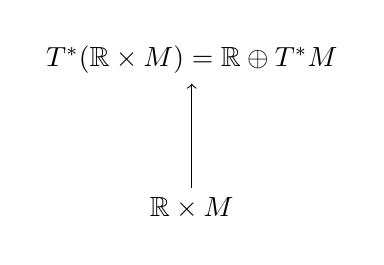
\begin{tikzpicture}
  \matrix (m) [matrix of math nodes, row sep=3.8em, column sep=4.8em, minimum width=2.2em]
  {
T^*(\mathbb{R} \times M) = \mathbb{R} \oplus T^*M \\
\mathbb{R} \times M \\
};
  \path[->]
  (m-2-1) edge node [auto] {$$} (m-1-1)
  ;
\end{tikzpicture} \text{ in that } 
\begin{tikzpicture}
  \matrix (m) [matrix of math nodes, row sep=3.8em, column sep=4.8em, minimum width=2.2em]
  {
\alpha = \alpha_0 dt + \alpha_M = \alpha_0 dt + (\alpha_M)_i dx^i \\
(t,x)  \\
};
  \path[->]
  (m-2-1) edge node [auto] {$$} (m-1-1)
  ;
\end{tikzpicture}
\]
in that $i$ runs through the indices for (some) local chart of $M$ \emph{only}, i.e. $i=1,2, \dots \text{dim}M=d$.  

Likewise, $\Omega^p(\mathbb{R} \times M) = \Omega^{p-1}(M) \oplus \Omega^p(M)$, in that 
\[
\begin{gathered}
 \forall \,  \alpha \in \Omega^p(\mathbb{R} \times M) \text{ then for $\mu = 0, 1, 2, \dots d$, $0$ standing in for $t\in \mathbb{R}$ of $\mathbb{R}\times M$, }\\ 
\alpha = \alpha_M dx^M = dt \wedge \alpha_I dx^I + \alpha_J dx^J \text{ where } \begin{aligned} & M = (\mu_1 \dots \mu_p) \quad & \mu_{\mu} = 0,1 \dots d \quad & \mu_1 < \dots < \mu_p \\
  & I = (i_1 \dots i_{p-1}) \quad & i_i = 1 \dots d \quad & i_1 < \dots < i_{p-1} \\
  & J = (j_1 \dots j_{p}) \quad & j_j = 1 \dots d \quad & j_1 < \dots < j_{p} 
\end{aligned} 
\end{gathered}
\]
and so, naming these components of $\alpha$ as 
\[
\begin{aligned}
  & \alpha^{p-1} \equiv \alpha_I dx^I \in \Omega^{p-1}(M) \\ 
  & \alpha^{p} \equiv \alpha_J dx^J \in \Omega^{p}(M) 
\end{aligned}
\]
Then $\forall \, \alpha \in \Omega^p(\mathbb{R} \times M)$, 
\begin{equation}\label{Eq:p-form}
\alpha = dt \wedge \alpha^{p-1} + \alpha^p
\end{equation}.  Taking $d$ on both sides to obtain $d\alpha \in \Omega^{p+1}(\mathbb{R} \times M)$, and $d\alpha$, being a $p+1$-form, taking the form of Eq. \ref{Eq:p-form}, then
\[
\begin{gathered}
  d\alpha = dt \wedge (d\alpha)^p + (d\alpha)^{p+1} = -dt \wedge d^{\perp} \alpha^{p-1} + \frac{ \partial \alpha^p_J}{ \partial t} dt \wedge dx^J + d^{\perp}\alpha^p
\end{gathered}
\]
where $d\alpha^p = \frac{ \partial \alpha^p_J}{ \partial x^{\mu }} dx^{\mu} \wedge dx^J = \frac{ \partial \alpha^p_J}{\partial t} dt \wedge dx^J + \frac{ \partial \alpha_J^p}{ \partial x^i} dx^i \wedge dx^J = \frac{ \partial \alpha_J^p }{ \partial t} dt \wedge dx^J + d^{\perp}\alpha^p$, and so $d^{\perp}$ signifies that this exterior derivative only ``acts'' on the (local) coordinates of $M$.  

Thus
\[
\begin{aligned}
  & (d\alpha)^p = -d^{\perp} \alpha^{p-1}  + \frac{ \partial \alpha^p }{ \partial t} \\ 
  &  (d\alpha)^{p+1} = d^{\perp}\alpha^p
\end{aligned}
\]

Suppose $\alpha = \psi^* \omega$; $\omega \in \Omega^p(N)$; $\psi : [0,1] \times M \to N$.  \\
If $\omega$ closed ($d\omega =0$), then $\psi^*\omega$ closed ($d\psi^* \omega = \psi^* d\omega =0$).  

So using the above facts shown for $\alpha = \psi^* \omega$,
\[
\begin{gathered}
\begin{aligned}
  & \alpha = dt \wedge \alpha^{p-1} + \alpha^p \xrightarrow{ \alpha = \psi^* \omega } \psi^* \omega = dt \wedge (\psi^* \omega)^{p-1} + (\psi^* \omega)^p \\ 
  &  d\psi^* \omega = \psi^* d\omega = 0 = dt \wedge (d\psi^* \omega)^p + (d\psi^* \omega)^{p+1}
\end{aligned} \\
\begin{aligned}
  &  (d\psi^* \omega)^{p+1} =0 = d^{\perp}(\psi^* \omega)^p \\ 
  & (d\psi^* \omega)^p = 0 = -d^{\perp}(\psi^* \omega)^{p-1} + \frac{ \partial ( \psi^* \omega)^p }{ \partial t} \xrightarrow{ \int_0^1 dt } \left. (\psi^* \omega)^p \right|_{t=1} - \left. (\psi^* \omega)^p \right|_{t=0} = d^{\perp} \int(\psi^* \omega)^{p-1} \text{ or } 
\end{aligned} \\
f_1^* \omega - f_0^* \omega = d^{\perp} \int (\psi^* \omega)^{p-1}
\end{gathered}
\]

So $f_1^* \omega$ differ from $f_0^* \omega$ by an exact form, $d^{\perp} \int(\psi^* \omega)^{p-1}$.  
\[
\Longrightarrow [f_1^* \omega] = [f_0^* \omega]
\]
Thus deRham cohomology classes are invariant under homotopy (homotopy invariant!).  

Consider 1-form connection on principal $G$-bundle $A=A(x) \in \Omega^1(M;\mathbf{g})$, $\forall \, x \in M$, $\mathfrak{g}$ Lie algebra of $G$ (Recall $\mathbf{g} = T_1G$).  \\
Consider 1-form connection over $[0,1] \times U$, open $U \subset M$, $A'=A'(t,x)$ in that
\[
A' = \mathbf{g}^{-1}d\mathbf{g} + t\mathbf{g}^{-1} A \mathbf{g} = A'(t,x)
\]
Note that $\mathbf{g} \in \mathfrak{g}$.  

$A'$ interpolates between a flat connection $A'(0,x) = \left. A' \right|_{t=0} = \mathbf{g}^{-1} d\mathbf{g}$, the connection 1-form for product principal bundle $P=M\times G$ and $A'(1,x) = \left. A'\right|_{t=1} = \mathbf{g}^{-1} d\mathbf{g} + \mathbf{g}^{-1} A \mathbf{g}$.  I think that this could be interpreted as turning off and turning on the gauge field, respectively.  

Now, doing the calculation out explicitly,
\[
\begin{gathered}
F_{A'} = (d+A')^2 = dA' + A'\wedge A' = d\mathbf{g}^{-1} \wedge d\mathbf{g} + dt \wedge \mathbf{g}^{-1} A \mathbf{g} + t(d\mathbf{g}^{-1} \wedge A \mathbf{g} + \mathbf{g}^{-1} dA \mathbf{g} + \mathbf{g}^{-1} A \wedge d\mathbf{g} + \\
 + t(\mathbf{g}^{-1} d\mathbf{g} \wedge \mathbf{g}^{-1} A \mathbf{g} + \mathbf{g}^{-1} A \mathbf{g} \wedge \mathbf{g}^{-1} d\mathbf{g} ) + t^2 \mathbf{g}^{-1} A \wedge A \mathbf{g}
\end{gathered}
\]
Using this identity:
\[
\begin{gathered}
  \mathbf{g}^{-1} \mathbf{g} = 1 \\ 
  \Longrightarrow d( \mathbf{g}^{-1} \mathbf{g} ) = d\mathbf{g}^{-1} \mathbf{g} + \mathbf{g}^{-1} d\mathbf{g} = 0 
\end{gathered}
\]
and ``commuting'' or ``moving through'' differential forms ``through the wedge product'', then
\[
F_{A'} = tdA + dt \wedge A + t^2 A \wedge A
\]

Now consider $\text{tr}(F_{A'} \wedge F_{A'} ) \in \Omega^4([0,1]\times U)$.  

$\text{tr}(F_{A'} \wedge F_{A'})$ is closed, since $\text{dim}M = 4$.  

Now recall that $\forall \, p$-form on $[0,1] \times U$, $\alpha \in \Omega^p([0,1]\times U)$, $\alpha = dt \wedge \alpha^{p-1} + \alpha^p$; with $\begin{aligned} & \quad \\ 
  & \alpha^{p-1} \in \Omega^{p-1}(U) \\
  & \alpha^p \in \Omega^p(U) \end{aligned}$

Thus, in our case currently, 
\[
\text{tr}(F_{A'} \wedge F_{A'}) = dt \wedge \alpha^3 + \alpha^4
\]
Calculating out $F_{A'} \wedge F_{A'}$ explicitly,
\[
\begin{gathered}
  F_{A'} \wedge F_{A'} = dt \wedge A \wedge tdA + t^3 A \wedge A \wedge dA + tdA \wedge dt \wedge A + t^2 dt \wedge A \wedge A \wedge A + \\
  + tdA \wedge A \wedge A + t^2 dt \wedge A \wedge A \wedge A =  \\
   = 2dt \wedge tA \wedge dA + 2 t^2 dt \wedge A \wedge A \wedge A + (t^3 + t) A\wedge A \wedge dA
\end{gathered}
\]
and so 
\[
\alpha^3 = 2\text{tr}(tA \wedge dA + t^2 A \wedge A \wedge A)
\]

Since $\text{tr}(F_{A'} \wedge F_{A'})$ closed, $0 = 0 - dt \wedge d\alpha^3 + d\alpha^4$, and ``applying'' $\frac{ \partial }{ \partial t}$ to this expression (i.e. this 4-form ``acts'' on $\frac{ \partial }{ \partial t}$, then 
\[
\begin{gathered}
  \frac{ \partial \alpha^4}{ \partial t} = d\alpha^3 \\ 
\xrightarrow{ \int dt } \int \frac{ \partial \alpha^4}{ \partial t} = \int d\alpha^3 = \text{tr}(F_{A'(1)} \wedge F_{A'(1)} ) - \text{tr}(F_{A'(0)} \wedge F_{A'(0) } ) = d\text{tr}(A\wedge dA + \frac{2}{3} A \wedge A \wedge A)
\end{gathered}
\]
Explicitly,
\[
\begin{gathered}
  d(\text{tr}(F_{A'} \wedge F_{A'}) ) = -dt \wedge d\alpha^3 + d\alpha^4 \\ 
  \xrightarrow{ \left( \frac{ \partial }{ \partial t} , \cdot, \cdot, \cdot \right) } \frac{ \partial ( \text{tr}(F_{A'} \wedge F_{A'} ) ) }{ \partial t} = - d\alpha^3 \xrightarrow{ \int_0^1 dt } \int_0^1 dt \frac{ \partial \text{tr}( F_{A'} \wedge F_{A'})}{ \partial t} = \int_0^1 dt ( -d\alpha^3)
\end{gathered}
\]
and so for $\text{tr}(F\wedge F) \in \Omega^4(M)$, $\text{tr}(A \wedge dA + \frac{2}{3} A \wedge A \wedge A) \in \Omega^3(M)$
\[
\Longrightarrow \text{tr}(F_A \wedge F_A) \equiv \text{tr}(F\wedge F) = d\text{tr}(A \wedge dA + \frac{2}{3} A \wedge A \wedge A )
\]
For oriented smooth $M$; $\text{dim}M=4$
\[
\int_M \text{tr}(F\wedge F)= \int_M d\text{tr}(A \wedge dA + \frac{2}{3} A \wedge A \wedge A ) = \int_{\partial M} \text{tr}(A \wedge dA + \frac{2}{3} A \wedge A \wedge A)
\]


From \emph{Wikipedia}, on ``Standard Model (mathematical formulation)'', (cf. \url{https://en.wikipedia.org/wiki/Standard_Model_(mathematical_formulation)}), they have a nice and neat chart of the field content of the standard model (SM) and I'll reproduce the gauge fields table:



Redi and Sato (2016) \cite{RS1602} gives a good overall review of the current status of axions in a theory context.

\begin{thebibliography}{9}

\bibitem{CTaubes2011}
Clifford Henry Taubes, \textbf{Differential Geometry: Bundles, Connections, Metrics and Curvature} (Oxford Graduate Texts in Mathematics, Vol. 23) Oxford University Press; 1 edition (December 1, 2011). ISBN-13: 978-0199605873


%\cite{Witten:1988hf}
\bibitem{Witten:1988hf} 
  E.~Witten,
  ``Quantum Field Theory and the Jones Polynomial,''
  Commun.\ Math.\ Phys.\  {\bf 121}, 351 (1989).
  doi:10.1007/BF01217730
  %%CITATION = doi:10.1007/BF01217730;%%
  %2286 citations counted in INSPIRE as of 24 Feb 2016


\bibitem{GW2011}
Davide Gaiotto, Edward Witten. \emph{Knot Invariants from Four-Dimensional Gauge Theory}. 2011.   \href{http://arxiv.org/abs/1106.4789}{arXiv:1106.4789 [hep-th]}


\bibitem{Hick2013}
Kevin Peter Hickerson.  \emph{The physics of ultracold neutrons and Fierz interference in beta decay.}  Dissertation (Ph.D.), California Institute of Technology. 2013.  \url{http://resolver.caltech.edu/CaltechTHESIS:11022012-135115177}


\bibitem{Guko2007}
Sergei Gukov.  ``Gauge theory and knot homologies.''  Fortschr. Phys. \textbf{55}, No. 5 – 7, 473 – 490 (2007) / \textbf{DOI} 10.1002/prop.200610385  \url{http://www.maths.ed.ac.uk/~aar/papers/gukov2.pdf}


\bibitem{RS1602}
Michele Redi, Ryosuke Sato. \emph{Composite Accidental Axions}. \href{arXiv:1602.05427 [hep-ph]}{arXiv:1602.05427} [hep-ph].  \url{http://arxiv.org/abs/1602.05427}


\end{thebibliography}

\end{document}

